\clearpage
\section{Domain Model}
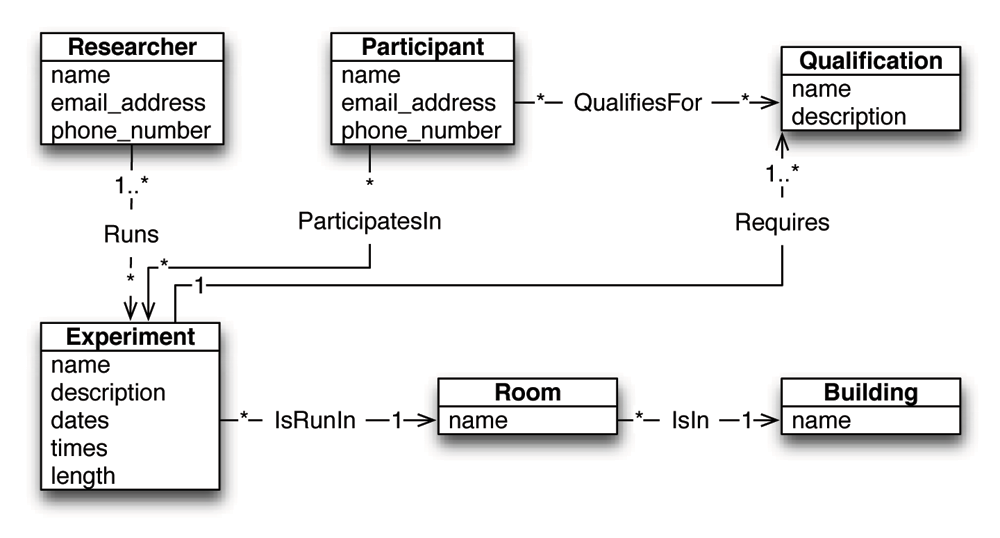
\includegraphics[width=7in]{../other/domain-model/domain-model}

The central entity in the Participant Scheduling System is the
\textbf{Experiment}. Each \textbf{Experiment} has a name, description,
length (in minutes), and dates and times it is run. Furthermore, each
\textbf{Experiment} is run in a \textbf{Room}, which has a name. Each
\textbf{Room} is in a \textbf{Building}, which also has a name.

For every \textbf{Experiment}, at least one \textbf{Researcher} runs
it. A \textbf{Researcher} has a name, email address, and phone number.
Any number of \textbf{Participants} participate in an
\textbf{Experiment}. Like a \textbf{Researcher}, a
\textbf{Participant} has a name, email address, and phone number.

Every \textbf{Experiment} requires at least one
\textbf{Qualification}. A \textbf{Qualification} has a name and
description. A \textbf{Participant} qualifies for a
\textbf{Qualification}.
